\documentclass[14pt,titlepage]{extbook}

\usepackage[latin1]{inputenc}
\usepackage[T1]{fontenc}
\usepackage[portuges]{babel}

\usepackage{amsmath,amsthm,amssymb}
\usepackage{mathtools,empheq}
\usepackage{verbatim,url}
\usepackage{epsfig}
\usepackage[bf]{subfigure}
\usepackage[bf]{caption}

\newtheorem{definition}{Defini��o}
\newtheorem{theorem}{Teorema}
\newtheorem{notation}{Nota��o}
\floatname{algorithm}{Algoritmo}

\usepackage{url}
\usepackage{hyperref}
\hypersetup{%
%  colorlinks=false,
%  citecolor=black,
   pagebackref=true,
   breaklinks=true,
   colorlinks,
   linktoc=all
}%

%\usepackage[numbers]{natbib}
\usepackage{natbib}

% For setmarginsrb:
\usepackage{vmargin}

\usepackage{nomencl}
\usepackage{fancyhdr}
\setlength{\headheight}{15.2pt}

% commutative diags
\usepackage{tikz-cd}

% customize lists
\usepackage{enumitem}

\renewcommand{\cite}{\citep}
%\newcommand{\mynewpage}{{\mbox{BLANK PAGE}}\cleardoublepage}
%\newcommand{\mynewpage}{{\mbox{}}\cleardoublepage}
\newcommand{\mynewpage}{}
% For onehalfspacing or doublespacing:
%\usepackage{setspace}

%%%%%%%%%%%%%%%%%%%%%%%%%%%%%%%%%%%%%%%%%%%%%%%%%%%%%%%%%%%%%%%%%%%%%%%%%%%%%%%

\includeonly{%
  front-matter,
  intro,
  todo,
  refs,
}

\renewcommand{\nomname}{Table of Notations}
\makenomenclature

% -- Possible lems.sty
% TODO - include new command for epheq/aligned eqn environments with braces
\renewcommand{\qedsymbol}{$\blacksquare$}
%%%%%%%%%%%%%%%%%%%%%%%%%%%%%%%%%%%%%%%%
% You have two versions of the macro
% \draftnote{My note}. The first version puts notes (e.g. My note in the example)
% into the margin of your document. The second formats the note as nothing. You
% 'comment out' the version of the macro you don't want (using a % at the
% beginning of the line).
\newcommand{\draftnote}[1]{\marginpar{\tiny\raggedright\textsf{\hspace{0pt}#1}}}
%\newcommand{\draftnote}[1]{}
%
% This one is just for the comments for in-line text.
\newcommand{\indraftnote}[1]{\textcolor{blue}{\texttt{\footnotesize [#1]}}}
\newcommand{\todo}[1]{\indraftnote{todo: #1}} % Este  "a fazer" � para eu n�o esquecer

\def\FigureFont{\footnotesize}
\def\TableFont{\small}
\def\SectionTitleFont{\large}
\def\TextFont{\normalsize}
\def\ReferenceFont{\normalsize}
\def\Reducefigspace{\vspace{-0.7 truecm}} %0.3
\def\ReduceRDfigspace{\vspace{-1.51truecm}}
\def\ReduceEndFigSpace{\vspace{-0.01 truecm}} %0.38
\def\ReduceRefSpace{\vspace{-0.01 truecm}} %0.5
\def\SectionSpacing{\vspace{0.5 truecm}} %0.25
\def\SubSectionSpacing{\vspace{0.5 truecm}} %0.25
\def\subsubsection#1{\par\medskip\noindent{\bf #1}\quad\nopagebreak}
\def\Bibspace{\vspace{-0.5cm}}
\def\ReduceSubsectionBelow{\vspace{-0.2cm}}
\def\ReduceSubsectionAbove{\vspace{-0.5cm}}
\def\IncreaseSubSubSectionAbove{\vspace{0.2cm}}
\def\ReduceEqSpace{\vspace{-0.1cm}}
\def\ReduceSecSpace{\vspace{-0.1cm}}


\newcommand{\etc}{{\it etc}}
\newcommand{\ie}{{\it i.e.}}
\newcommand{\eg}{{\it e.g.}}
\newcommand{\wrt}{{\it w.r.t. }}
\newcommand{\etal}{{\it et.~al.}}
\newcommand{\intinf}{\int_{-\infty}^{\infty}}
\newcommand{\grad}{\nabla}
\newcommand{\slant}{\sigma}
\newcommand{\R}{\mathbb{R}} % the reals
\newcommand{\trace}{\text{trace}\,}
%\newcommand{\det}{\text{det}}

% skew-symmetric arrangement
\newcommand{\skewm}[1]{{#1}_\times}

\renewcommand{\vec}[1]{\mathbf{#1}}

\newcommand{\lbar}{\overline}

\newcommand{\id}{\text{\emph{I}}}
\newcommand{\dof}{\textsc{dof}}
\newcommand{\ransac}{\textsc{ransac}}
\newcommand{\sift}{\textsc{sift}}
\newcommand{\klt}{\textsc{klt}}
\newcommand{\svd}{\textsc{svd}}
\newcommand{\sfm}{\textsc{sfm}}
\newcommand{\rot}{\mathcal{R}}
\newcommand{\brot}{\overline{\mathcal{R}}}

\def\bsq#1{%both single quotes
\lq{#1}\rq}

% The following are not very good constructs it seems. Better to use just
% \begin{bmatrix}..\end{\bmatrix}

\newcommand{\datsqbr}[2][rrrrrrrrrrrrrrrrrrrrrrrrrrrrrrrrrrrr]{\left[
\begin{array}{#1}
#2\\
\end{array}
\right]
}


% -- !lems.sty

%%%%%%%%%%%%%%%%%%%%%%%%%%%%%%%%%%%%%%%%%%%%%%%%%%%%%%%%%%%%%%%%%%%%%%%%%%%%%%%
%\setmarginsrb{30mm}{27mm}{20mm}{20mm}{12pt}{25pt}{0pt}{5mm}
\setmarginsrb{20mm}{27mm}{20mm}{25mm}{12pt}{25pt}{0pt}{10mm}
%             left   top  right bottom headheight headsep footheight footsep 


\newtheorem{thm}{Theorem}
\newtheorem{lem}[thm]{Lemma}

\newtheorem{theorem}{Theorem}[section]
\newtheorem{corollary}[theorem]{Corollary}
\newtheorem{corolary}[theorem]{Corollary}
\newtheorem{proposition}[theorem]{Proposition}
\newtheorem{lemma}[theorem]{Lemma}

\theoremstyle{definition}
\newtheorem{definition}{Definition}
\newtheorem{remark}{Remark}[section]
\newtheorem{problem}{Problem}[section]
\newtheorem{question}{Question}[section]
\newtheorem{property}{Property}
\newtheorem{example}{Example}
\newtheorem{transformation}{Transformation}

\numberwithin{equation}{section}

\newcommand{\Gama}{\boldsymbol{\Gamma}}
\newcommand{\gama}{\boldsymbol{\gamma}}
\newcommand{\gamad}{\dot{\gama}}
\newcommand{\bsigma}{\boldsymbol{\sigma}}
\newcommand{\T}{\boldsymbol{T}}
\newcommand{\N}{\mathbf{N}}
\newcommand{\NSurface}{\mathbf{N}}
\newcommand{\Nlocal}{\overline{\N}} % normal in local coordinates
\newcommand{\balpha}{\boldsymbol{\alpha}}
\newcommand{\tDt}{t+\Delta t}
\newcommand{\bpsi}{\boldsymbol{\boldsymbol{\psi}}}
\newcommand{\bp}{\mathbf p}
\newcommand{\deldt}[1]{\frac{\partial#1}{\partial t}}
\newcommand{\ddt}[1]{\frac{d #1}{dt}}
\newcommand{\delds}[1]{\frac{\partial#1}{\partial s}}
\newcommand{\mybar}[1]{\overline{#1}}
\newcommand{\norm}[1]{\|#1\|}
\newcommand{\I}{\mathbf{I}}
\newcommand{\brho}{\boldsymbol{\rho}}
\newcommand{\lightrgb}{\boldsymbol{l}}
\newcommand{\B}{\boldsymbol{B}}
\renewcommand{\t}{\boldsymbol{t}}
\newcommand{\n}{\boldsymbol{n}}
\renewcommand{\b}{\boldsymbol{b}}
\newcommand{\e}{\boldsymbol{e}}
\newcommand{\f}{\boldsymbol{F}}
\newcommand{\hf}{\boldsymbol{\hat{f}}}
\newcommand{\g}{\boldsymbol{g}}
\newcommand{\G}{\boldsymbol{G}}
\newcommand{\bc}{\boldsymbol{c}}
\newcommand{\Curve}{\boldsymbol{\mathcal{C}}}
%\newcommand{\X}{\boldsymbol{X}}
%\newcommand{\x}{\boldsymbol{x}}
\newcommand{\X}{\mathbf{X}}
\newcommand{\x}{\mathbf{x}}
\newcommand{\xx}{\mathcal{X}}  % used in Giblin's notes
\newcommand{\tilx}{\tilde x}
\newcommand{\tily}{\tilde y}
\newcommand{\tilgama}{\tilde \gama}
\newcommand{\ugama}{\hat{\gama}} %unit gama
\newcommand{\br}{\bar r}
\newcommand{\Kc}{\mathbf K_c}
\newcommand{\lepi}{\mathbf r}
\newcommand{\itan}{\tan^{-1}}
\newcommand{\uu}{\xi}
\newcommand{\buu}{\bar \uu}
\newcommand{\bvv}{\bar \vv}
\newcommand{\vv}{\eta}
\newcommand{\VV}{\mathbf{V}} % translational velocity
\newcommand{\VVspeed}{V} % translational velocity
\newcommand{\field}{\boldsymbol\chi}
\newcommand{\ufield}{\hat{\boldsymbol{\chi}}}
\newcommand{\fieldc}{\chi} % field component
\newcommand{\transl}{\mathcal{T}} % field component
\newcommand{\btransl}{\overline{\mathcal{T}}} % field component
\newcommand{\albedo}{\alpha}
\newcommand{\depth}{\rho}      % depth as z
\newcommand{\ddepth}{\dot{\rho}}      % depth as z
\renewcommand{\l}{\lambda} % used in problem2-thoughts-giblin
\newcommand{\udepth}{{\hat{\rho}}} % depth along ray
\newcommand{\ttransl}{\T} % translation tangent
\newcommand{\surface}{\mathcal{M}} % surface/manifold
\newcommand{\surf}{\mathcal{M}} % surface/manifold short
\newcommand{\jacm}{\mathtt{J}} % Jacobian matrix
\newcommand{\xbar}{\bar x}
\newcommand{\ybar}{\bar y}
\newcommand{\zbar}{\bar z}

\newcommand{\bdelta}{\boldsymbol \delta}
%\newcommand{\X}{\boldsymbol{X}}
%\newcommand{\x}{\boldsymbol{x}}
%\newcommand{\X}{\mathbf{X}}
%\newcommand{\x}{\mathbf{x}}
\newcommand{\boldu}{\mathbf{u}}
\newcommand{\boldv}{\mathbf{v}}
\newcommand{\boldw}{\mathbf{w}}
\newcommand{\tgtveloc}{\tilde\alpha} % real tangential velocity

\makeindex
\setcounter{tocdepth}{1}

\addto\captionsenglish{\renewcommand{\chaptername}{Lecture}}
\addto\captionsportuges{\renewcommand{\chaptername}{Aula}}

\begin{document}

%\authorrunning{Fabbri and Kimia}
%\mynewpage
%\listoffigures
%\onehalfspacing
\begin{titlepage}
\begin{center}

 % \vspace*{0.4cm}

 % \includegraphics[width=2.5cm, height=2.5cm]{v1.png}

\includegraphics[height=1.5cm]{figs/iprj-heading-v1.png}
  \vspace{2cm}

%\begin{minipage}[b]{12cm}\noindent
%    \begin{center}
%      {\Large Universidade do Estado do Rio de Janeiro} \\ {\Large
%	Instituto Politécnico - \Large IPRJ}
%    \end{center}
%  \end{minipage}

 % \Large

  %\sffamily

  %\vspace{0.4cm}

\begin{center}
 % {\LARGE \textbf{Método de redução de dimensionalidade não linear: um estudo sobre aplicação de difusão}}
% {\huge \textbf {Um estudo de redução de\vskip1cm
 %  dimensionalidade  por difusão}} \vskip1cm
  {\huge \textbf {Álgebra Linear Numérica }}
  \vskip1cm 
 
\end{center}

  \vspace{0.6cm}
  {\LARGE \textbf{Notas de Aula}}

\vspace{10 cm} % eu coloquei este que não tinha

\begin{center}
\textbf{Ricardo Fabbri}
\end{center}


 \begin{center}
  \vspace{0.5 cm}
 
% \usdate
 {\large \textbf{\today}}%\currenttime}}
\end{center}
\end{center}
\end{titlepage}
\thispagestyle{empty}
\frontmatter

%\tableofcontents
%\listoffigures
%\printnomenclature[3.5cm]
\mainmatter
\pagestyle{fancy}
\fancyhead[LE]{\nouppercase{\leftmark}}
\fancyhead[RE]{\thepage}
\fancyhead[LO]{\nouppercase{\rightmark}}
\fancyhead[RO]{\thepage}
\mynewpage
\chapter{O que � uma matriz?}

\section*{Objetivos}
\begin{itemize}
\item Aula introdut�ria informal dando vis�o geral e uma contextualiza��o do curso
\item Motivar alunos de engenharia da computa��o da import�ncia da disciplina ao
  final do curso, no contexto de modelagem computacional do IPRJ/UERJ.
\item O que � �lgebra linear num�rica: explicar termos ``�lgebra'', ``linear'',
  e ``num�rica''. Por qu� s�o importantes.
\item Matrizes como representa��o num�rica de transforma��es lineares
\item Crit�rio de avalia��o
\end{itemize}

\subsection*{O que � uma matriz?}
\begin{itemize}
\item Uma tabela retangular de n�meros, por�m n�o s�. 
\item Associados � tabela h� uma ``�lgebra'': opera��es alg�bricas
  usuais de multiplica��o matriz-vetor e matriz-matriz vistas no ensino m�dio,
  que parecem arbitr�rias.
\item Quando falamos de matrizes em engenharia e ci�ncia, sempre incluimos, portanto, tais opera��es.
\item O curso se chama �lgebra Linear Num�rica. At� agora, ent�o, falamos algo
  de ``num�rico'' (matrizes s�o um monte de n�meros) e de ``alg�bra''
  (opera��es). E o ``linear''?
\item Matrizes s�o representa��es num�ricas de transforma��es lineares.
\end{itemize}

\subsection*{O que � ``Linear''?}
\begin{itemize}
\item Ao ouvir a palavra ``linear'', a maioria das pessoas tem em mente uma reta ou um
plano.
\item ``Linearidade'' em matem�tica � uma forma de ``simplicidade''.
\item Esta simplicidade se manifesta em diversos n�veis: o geom�trico, o
  simb�lico, e o num�rico:
\end{itemize}
   
\paragraph{Simb�lico:}
No plano simb�lico ou alg�brico, explica-se os fen�menos de forma operacional e
abstrata, sem muita intui��o conceitual sobre o significado dos s�mbolos ou opera��es.
\begin{defi} \emph{(Simbolicamente Linear)} \label{def:linear:symbolic}
Muitos matem�ticos ir�o definir ``linear'' como a
  qualidade de uma fun��o ou transforma��o $L$ tal que 
  \begin{empheq}[left=\empheqlbrace]{align}
    &L(v + w) = L(v) + L(w)\\
    &L(\alpha v) = \alpha L(v),
    \label{eq:linear:symbolic}
  \end{empheq}
  para todos vetores $v$ e $w$, e escalares $\alpha$.
\end{defi}
\begin{itemize}
\item Tal defini��o, apesar de suscinta e formalmente elegante, tem pouca
  concretude imediata.
\item ``Linear'' aqui significa apenas uma simplicidade formal, ou seja, as
  manipula��es alg�bricas s�o simples.
\end{itemize}

\paragraph{Geom�trico:} No plano que aqui chamamos de ``geom�trico'',
``conceitual'', ou ``visual'', os fen�menos s�o explicados de maneira concreta,
mais pr�xima do objetivo ou de aplica��es reais. 

No mundo real, o que observamos
a princ�pio n�o � num�rico nem simb�lico: uma bola girando, um fl�ido em movimento, ou um feixe de n�utrons.
Muitas vezes, conceitos pr�ximos da realidade, independentes das conven��es de s�mbolos ou
n�meros, s�o dif�ceis de formalizar e, portanto, n�o s�o enfatizados na maioria
dos cursos de �lgebra linear.
\begin{defi} \emph{(Geometricamente Linear)}
  Chama-se ``Linear'' qualquer opera��o geom�trica que combina quaisquer das seguintes
  opera��es simples: girar, esticar e refletir.
  \label{def:linear:geometric}
\end{defi}

\begin{itemize}
\item Tais opera��es s�o globais e realizadas sobre um mesmo ponto central (origem)
\item O esticamento pode ser realizado por fatores diferentes ao longo de eixos arbitr�rios, e inclui achatamentos
\item Geralmente, esta defini��o � um teorema na teoria da �lgebra linear, visto
  apenas no final de um primeiro curso.  Trata-se
  do teorema do SVD -- \emph{Singular Value Decompositon}, ou decomposi��o em
  valores singulares. Trata-se de um an�logo de autovalores e autovetores, e � o
  teorema mais importante a ser explorado neste curso.
\item Como exemplo, temos a seguinte figura:
  \begin{center}
  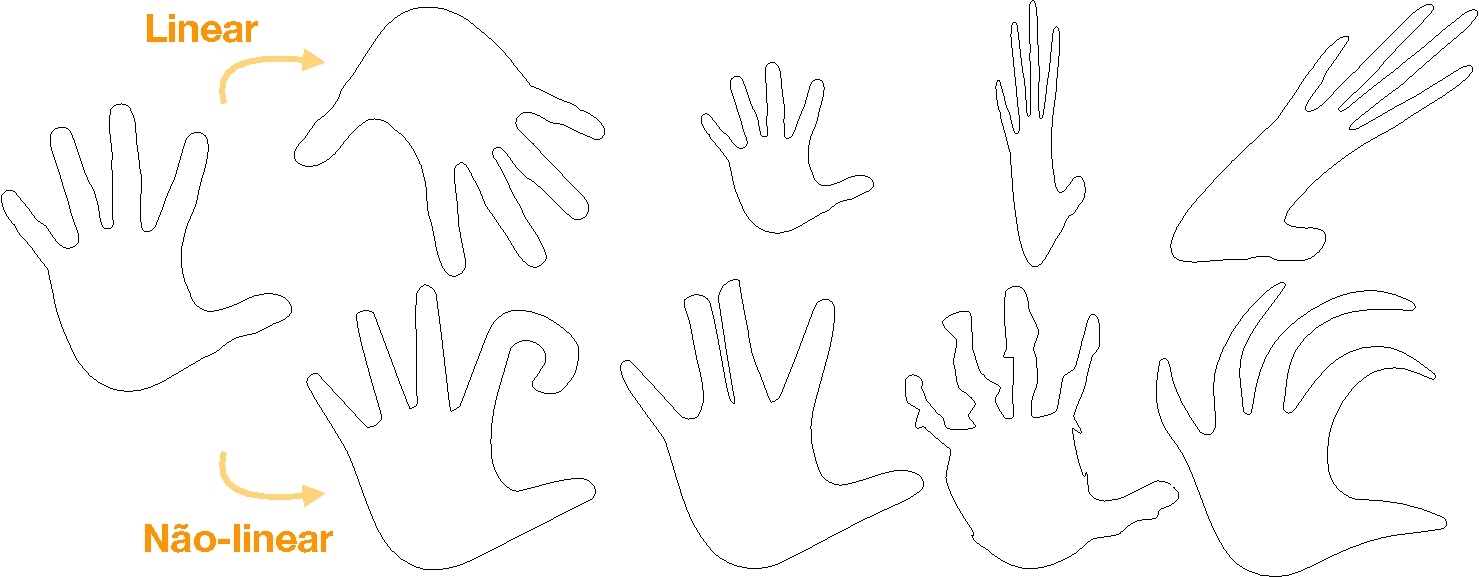
\includegraphics[scale=0.5]{figs/nonlinear-transf-hands.pdf}
  \end{center}
  A m�o � esquerda sofre transforma��es lineares na linha acima, e n�o-lineares
  na linha abaixo. As transforma��es acima s�o lineares pois consistem em
  girar ou esticar cada ponto da m�o globalmente pelo mesmo �ngulo ou fatores de
  esticamento. J� as transforma��es na linha abaixo s�o n�o-lineares pois os
  pontos ou sofrem deforma��es locais (diferentes para cada ponto da m�o), ou
  n�o s�o meramente girados e esticados.
\end{itemize}

\paragraph{Num�rico:} J� definimos no in�cio da aula que uma matriz � a
representa��o num�rica de uma transforma��o linear, seja esta pensada pela
defini��o geom�trica ou simb�lica. 
\begin{itemize}
\item Para maior compreens�o do significado dos n�meros e opera��es de uma
  matriz, na pr�xima aula revisaremos o conceito de \emph{coordenadas}.
\item Tamb�m revisaremos como encontrar os n�meros em uma matriz para uma dada
  transforma��o linear
\end{itemize}
O teorema do SVD pode ser descrito num�ricamente em termos de matrizes:
\begin{teo}\label{teo:svd:informal}
  (SVD numerico - informal)
  Toda matriz A de tamanho $m\times n$ pode ser escrita da forma:
  \begin{center}
  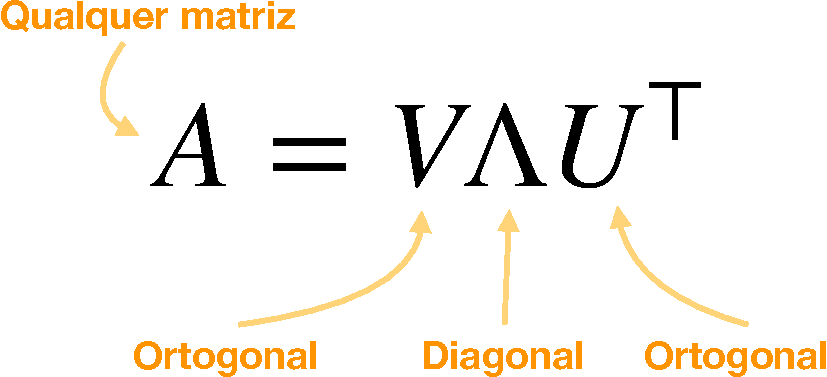
\includegraphics[scale=0.5]{figs/svd-matricial.pdf}
  \end{center}
  Ou seja, toda matriz � uma matriz diagonal junto com matrizes ortogonais.
  A matriz diagonal realiza esticamento em cada eixo, e as matrizes ortogonais
  realizam rota��es e reflex�es. 
\end{teo}
\begin{itemize}
\item O tamanho das matrizes �
  \begin{equation}
   A_{m\times n} = V_{m\times m}\,\Lambda_{m\times n}\, U_{n \times n}^\top 
  \end{equation}
\item Portanto toda matriz �, de certa forma, equivalente a uma matriz diagonal de mesmo
  tamanho.
\item Matrizes diagonais s�o matrizes da seguinte forma (exemplo $3\times 3$):
  \begin{equation}
    \Lambda = 
    \begin{bmatrix}
     a & 0 & 0 \\
     0 & b & 0 \\
     0 & 0 & c \\
   \end{bmatrix},
    \label{eq:diagonal}
  \end{equation}
  as quais transformam pontos $(x,y,z)$ da seguinte forma:
  \begin{equation}
    \Lambda = 
    \begin{bmatrix}
     a & 0 & 0 \\
     0 & b & 0 \\
     0 & 0 & c \\
    \end{bmatrix}
    \begin{bmatrix}
      x\\
      y\\
      z
    \end{bmatrix}
    = 
    \begin{bmatrix}
      a x\\
      b y\\
      c z
    \end{bmatrix},
  \end{equation}
  ou seja, esticam cada ponto ao longo de eixos por fatores $a$, $b$ e $c$. 
\item Cada fator de esticamento $a$, $b$ ou $c$ pode ser zero, o que faz com que
  a matriz achate completamente uma das dimens�es
\end{itemize}

\paragraph{Observa��es}
\begin{itemize}
\item A transla��o � n�o-linear. Pode-se mostrar que, mesmo sendo uma opera��o
  geom�trica simples, a transla��o n�o tem as propriedades de simplicidade
  alg�brica como na defini�ao simb�lica acima, e tamb�m n�o pode ser expressa
  numericamente como uma multiplica��o de matrizes. 
\item Com alguns artif�cios, � poss�vel realizar transla��o com multiplica��o de matrizes,
  por�m � preciso opera��es n�o-lineares (proje��o).
\end{itemize}

\paragraph{Para qu� servem as transforma��es lineares, se elas s�o t�o
limitadas?}

\begin{itemize}
\item O mundo real � n�o-linear
\item O ``Linear'' foi inventado como uma simplifica��o do n�o-linear, mas em si
  n�o tem aplica��o pr�tica.
\item O linear n�o faz sentido sem o n�o-linear. 
\item O linear s� existe como artefato para modelar o n�o-linear.
\item O paradigma � tomar um fen�meno real (e n�o-linear) e lineariz�-lo, para
  usar as ferramentas deste curso.
\item Em C�lculo 1, estudamos fun��es n�o-lineares de uma vari�vel usando
  a derivada como lineariza��o local (reta tangente). A reta tangente � uma
  transforma��o linear de uma vari�vel.
\item Da� a import�ncia de se estudar cursos como an�lise no $\mathbb R^n$, onde
  fen�menos n�o-lineares s�o modelados tendo como
  ferramenta b�sica a �lgebra linear.
\item �lgebra linear tamb�m � o primeiro contato do aluno com $n$ dimens�es,
  para $n > 3$, e tem import�ncia direta na pr�tica, por exemplo em intelig�ncia artificial,
\emph{machine learning}.
\item Por exemplo, o paradigma de c�lculo e an�lise no $\mathbb R^n$ � estudar o
  n�o-linear realizando lineariza��es locais (diferencia��o). Dessa forma, para
  se deformar a m�o de forma mais geral, como na figura abaixo, pode-se usar
  v�rias transforma��es lineares com fatores de esticamento e rota��o diferentes para cada ponto:
  \begin{center}
  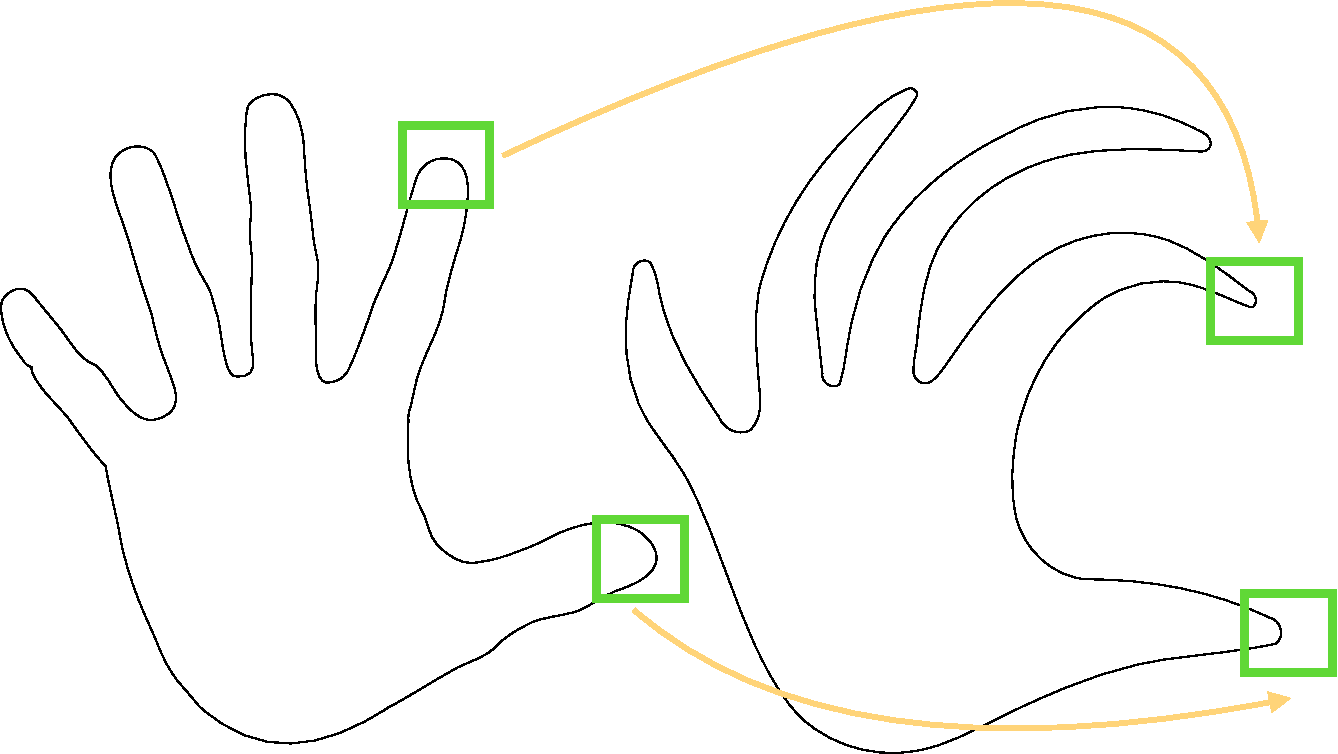
\includegraphics[scale=0.5]{figs/nonlinear-using-linear.pdf}
  \end{center}
\item Em cada quadrado verde, temos uma deforma��o pr�xima de uma rota��o e um
  esticamento.
\item Curiosidade: a deforma��o n�o-linear da m�o � uma fun��o de $\mathbb R^2
  \to \mathbb R^2$ estudada em An�lise no $\mathbb R^n$. A aproxima��o da
  deforma��o de cada quadrado verde � chamada de diferencial da fun��o
  n�o-linear, e sua forma num�rica (matricial) � estudada em �lgebra linear
  num�rica.
\end{itemize}

\subsection*{Tarefas}

\begin{itemize}
\item Site: \url{http://wiki.nosdigitais.teia.org.br/ALN}
\item Realizar tarefa 0 e tarefa 1 (datas no site).
\end{itemize}

\subsection*{Exerc�cios}
\begin{enumerate}
\item Explique como uma fun��o $f: \mathbb R \to \mathbb R$, $y = f(x)$, seria
  considerada linear, tanto em termos s�mb�licos e geom�tricos. Qual seria a
  f�rmula dessa fun��o?
\end{enumerate}

\mynewpage
\chapter{Revis�o de �lgebra Linear}

\section*{Objetivos}
\begin{itemize}
\item Relebrar representa��o num�rica de transforma��es lineares
\item Revisar �lgebra linear n�o-num�rica (``simb�lica'')
\item Estilo: revis�o aprofundada para alunos que ja viram a disciplina. Nota��o
solta adequada a uma revis�o.
\end{itemize}

\section*{Observa��es Iniciais}
\begin{itemize}
\item A �lgebra liner num�rica come�a com o conceito de escalares e coordenadas.
\item Para haver coordenadas, � necess�ria a escolha da escolha de uma base
\item O conceito de espa�o vetorial (simb�lico) permite isolar as opera��es
  que n�o dependem da escolha de uma base, daquelas que dependem.
\end{itemize}

\begin{defi} \emph{(Espa�o Vetorial Simb�lico)}
Um espa�o vetorial $\mathcal V$ sobre um corpo $K$ � uma tupla ordenada
$\mathcal V = (V, K, +, \cdot)$ de quatro elementos:
\begin{empheq}[left=\mathcal V\ \ \empheqlbrace]{align}
  &V\text{: conjunto cujos elementos s�o chamados ``vetores''}\nonumber\\
  &K\text{: conjunto cujos elementos s�o chamados ``escalares''}\nonumber\\
  &+\text{: soma de vetores}\nonumber\\
  &\cdot\text{: multiplica��o vetor-escalar,}\nonumber
\end{empheq}
onde ``+'' satisfaz:
\begin{align}
  +: V \times V &\to V\\
  (v,w) &\mapsto v+w,
\end{align}
\begin{align}
  &v + w = w + v\\
  &v + (u + w) = (v + u) + w\\
  &\exists !\ 0 \in V \text{ tal que } 0 + v = v,\ \forall v\in V\\
  &\forall v \in V, \exists !\ w \in V \text{ tal que } v + w = 0, \text{simbolizado por } -v
\end{align}
e onde ``$\cdot$'' satisfaz:
\begin{align}
  \cdot: K \times V &\to V\\
  (\alpha,w) &\mapsto v+w,
\end{align}
\begin{align}
  &v + w = w + v\\
  &v + (u + w) = (v + u) + w\\
  &\exists !\ 0 \in V \text{ tal que } 0 + v = v,\ \forall v\in V\\
  &\forall v \in V, \exists !\ w \in V \text{ tal que } v + w = 0, \text{simbolizado por } -v
\end{align}
e $K$ satisfaz as propriedades de uma estrutura alg�bridca chamada ``corpo'',
que abstrai as opera��es de multiplica��o, soma, subtra��o e divis�o poss�veis
com n�meros, geralmente $\mathbb R$ ou $\mathbb C$.
\end{defi}

\begin{itemize}
\item Aos programadores em C++: a defini��o de espa�o vetorial simb�lico � como uma
  \emph{classe}, que define as partes e as opera��es permitidas. 
\item Na defini��o simb�lica um vetor � apenas caracterizado pelas opera��es que
  se pode realizar com ele, e as propriedades de tais opera��es.
\item At� o momento, a �nica coisa ``num�rica'' nesta defini��o � o  
  corpo de escalares $K$. Os vetores ainda s�o entidades simb�licas que podem ser somadas e
  multiplicadas por escalar.
\item A teoria simb�lica parece artificialmente trivial -- todos j� sabemos as
  propriedades convencionais de soma de vetores e multiplica��o por
  escalar. 
\item No entanto, a teoria simb�lica est� mais pr�xima do conceitual que a
  teoria num�rica, pois isola os fatores que n�o dependem da escolha de um
  sistema de coordenada.
\item A conex�o com o mundo num�rico consiste em associar n�meros a vetores.
  Para tanto, � importante definir base e, para isso, depend�ncia linear.
\item Iremos assumir que $V$ e $W$ s�o espa�os vetoriais.
\end{itemize}

\begin{defi}
  Uma combina��o linear de $v_1,\dots,v_n$, $v_i \in V$, � uma express�o da
  forma
  \begin{equation}
    \alpha_1 v_1 + \dots + \alpha_n v_n = \sum \alpha_i v_i.
  \end{equation}
\end{defi}
\begin{itemize}
\item Nota��o: quando n�o h� ambuguidade, iremos omitir os �ndices dos
  somat�rios $\sum$.
\end{itemize}
\begin{defi}
  Os vetores $v_1,\dots,v_n$ s�o ditos linearmente indepententes (L.I.) se
  \begin{equation}
    \sum \alpha_i v_i\ \  \iff\ \  \alpha_i = 0\,\ i=1,\dots,n
  \end{equation}
\end{defi}

\begin{prop}
  $v_1,\dots,v_n$ s�o L.I. se, e somente se, cada $v_i$ n�o � o vetor nulo (isto
    �, $v_i \neq 0$) e nenhum � combina��o linear dos demais 
\end{prop}

\begin{defi}
  $\{v_1,\dots,v_n\} \subset V$ � base de $V$ se
\begin{empheq}[left=\empheqlbrace]{align}
  &v_1,\dots,v_n \text{ s�o L.I. e}\\
  &\text{todo $v \in V$ � combina��o linear dos $v_i$'s}
\end{empheq}
\end{defi}

Finalmente, chegamos ao conceito de coordenadas (num�ricas) de um vetor:
\begin{defi} \emph{(Coordenadas)} Dada uma base $B = \{v_1,\dots,v_n\}$ de $V$,
ent�o os n�meros $\alpha_1,\dots,\alpha_n$ tal que
  \begin{equation}
    v = \sum \alpha_i v_i
  \end{equation}
  s�o chamados de coordenadas de $v$ em $V$ (na base $B$). Quando necess�rio,
  utiliza-se a nota��o expl�cita: 
  \begin{equation}
  \mathcal X_B(v) = 
  \begin{bmatrix}
    \alpha_1\\
    \alpha_n
  \end{bmatrix},
  \end{equation}
  onde o s�mbolo ``chi'' $\mathcal X$ dever ser lido como ``coordenada de''.
\end{defi}

\begin{itemize}
\item Se pensarmos no vetor simb�lico $v\in V$ visualmente como uma seta desenhada no plano, suas
coordenadas s�o um vetor num�rico $2$ n�meros, sendo necess�rio definir a base
(posi��o dos eixos $x$ e $y$).
\item Fixada uma base, existe uma rela��o 1-1 entre vetores simb�licos $v$ e
  vetores de $n$ n�meros.
\end{itemize}

\begin{teo}
  Dada uma base de $n$ vetores, tem-se que:
  \begin{itemize}
  \item As $n$ coordenadas de um vetor s�o �nicas
  \item Qualquer outra base de $V$ tem o mesmo n�mero de elementos $n$, que usaremos como
    a defini��o da dimens�o de $V$.
  \end{itemize}
\end{teo}
\dem
Ambos decorrem de propriedades de sistemas lineares. Os detalhes j� foram
vistos pelo aluno no primeiro curso de �lgebra linear.
\fim


\mynewpage
\chapter{To Do}
\begin{enumerate}
\item Explicar melhor como retas e planos sao nao-lineares
\item Figura de transforma��es nao-lineares e nao-diferenciaveis (rasgar, formar
  bicos, etc)
\item enviar para daiara, carlos, francisco
\item Aula: Transformacoes rigidas: Rotacao e translacao
\item Aula: Coordenadas homogeneas
\item Aula: QR householder, QR givens
\item Aula: Cholesky
\item Aula: SVD: teorema e demonstracao, algumas figs, relembrar autovalores
\item Aula: homogeneizacao de sistemas e uso de SVD sobredeterminado
\item Aula: Aplicacao em imagens
\item Aula: Aplicacao em cameras
\item Aula: Aplicacao em reconhecimento
\end{enumerate}

\mynewpage
\bibliographystyle{plainnat}
%\bibliographystyle{authordate}
\bibliography{shading,multiview,motion,Kimia,bib-header,video,math-books,math,psych-books,metric,edge,leymarie_pami_scaffold,vision-books,vision,recognition,optical-flow,indexing,proceedings}


\end{document}
